\documentclass[10pt,a4paper]{article}

% -------------------------------------------------
% OSNOVNI PAKETI
% -------------------------------------------------
\usepackage[utf8]{inputenc}
\usepackage[T1]{fontenc}
\usepackage[croatian]{babel}
\usepackage{bookmark}
\usepackage{lmodern}
\usepackage{geometry}
\geometry{margin=1.8cm}

\usepackage{enumitem}
\usepackage{xcolor}
\usepackage{graphicx}
\usepackage{booktabs}
\usepackage{array}
\usepackage{hyperref}
\usepackage{listings}
\renewcommand{\lstlistingname}{Pseudokod}
\usepackage{tikz}
\usetikzlibrary{arrows.meta,positioning,shapes.geometric}

\hypersetup{
	colorlinks=true,
	linkcolor=blue,
	urlcolor=blue
}

\setlength{\parindent}{0pt}
\setlength{\parskip}{4pt}

\setlist[itemize]{
	topsep=2pt,
	itemsep=1pt,
	leftmargin=1.2em
}

\setlist[enumerate]{
	topsep=2pt,
	itemsep=1pt,
	leftmargin=1.4em
}

% -------------------------------------------------
% POSTAVKE ZA KOD
% -------------------------------------------------
\definecolor{codebg}{RGB}{245,245,245}

\lstset{
	basicstyle=\ttfamily\small,
	backgroundcolor=\color{codebg},
	frame=single,
	breaklines=true,
	columns=fullflexible
}

% -------------------------------------------------
% POSTAVKE ZA DIJAGRAME
% -------------------------------------------------
\definecolor{darkblue}{RGB}{30,70,130}

\tikzset{
	block/.style={
		rectangle,
		rounded corners,
		draw=darkblue,
		fill=blue!5,
		align=center,
		minimum height=8mm,
		text width=34mm
	},
	decision/.style={
		diamond,
		aspect=2,
		draw=red!70!black,
		fill=red!6,
		align=center,
		text width=25mm,
		inner sep=1pt
	},
	line/.style={-Latex,thick}
}

% -------------------------------------------------
% PODACI O SEMINARU
% -------------------------------------------------
\title{
	\textbf{ESP32 web dijagnostički terminal za Micromouse robota preko UART-a}\\[2mm]
	\large Programiranje mikrokontrolerskih sustava
}

\author{
	David Mihić\\
	Mehatronika i robotika
}

\date{
	Ljetni semestar 2026.
}

\begin{document}

\maketitle

\begin{center}
	\textbf{Mentor:} doc.\ dr.\ sc.\ Matija Krznar
\end{center}

\newpage

% -------------------------------------------------
\section*{1. Cilj projekta}
% -------------------------------------------------

Cilj projekta je dijagnostički modul (dashboard) na ESP32 mikrokontroleru koji služi kao web sučelje između operatera i Micromouse robota. Robot je izgrađen oko STM32G474 mikrokontrolera i preko UART-a kontinuirano šalje telemetriju. ESP32 te podatke prima, podiže vlastitu Wi-Fi pristupnu točku i poslužuje web stranicu na kojoj operater vidi stanje robota i može mu slati naredbe. Ne treba dodatni alat ni kabel prema računalu: operater se spoji na Wi-Fi mrežu robota i otvori stranicu u pregledniku.

Konkretno:
\begin{itemize}
	\item Sustav prikazuje stanje robota uživo: IR senzore, žiroskop, odometriju, brzine kotača, pozu, stanje tipki, DIP prekidača i Neopixel LED diode.
	\item Rješava se problem otklanjanja grešaka na robotu bez žičanog spoja na računalo i bez prekida rada robota.
	\item ESP32 je posrednik (bridge): pretvara UART vezu prema robotu u Wi-Fi i HTTP koji preglednik razumije.
	\item Korisnik može gledati telemetriju i slati naredbe (npr.\ reset odometrije) kroz serijsku konzolu na stranici.
\end{itemize}

% -------------------------------------------------
\section*{2. Funkcionalni zahtjevi}
% -------------------------------------------------

\begin{itemize}
	\item Uspostaviti UART komunikaciju između ESP32 i STM32 robota.
	\item Konfigurirati UART parametre: 115200 bit/s, 8 podatkovnih bitova, bez pariteta, 1 stop bit (8N1).
	\item Primati poruke s UART-a, sastavljati ih u cijele linije i činiti ih dostupnima web sloju.
	\item Omogućiti slanje tekstualnih naredbi s web stranice prema robotu preko UART-a.
	\item Prikazati status komunikacije (živa veza / nema podataka).
	\item Parsirati dogovoreni format telemetrije (JSON linija) i prikazati polja u odvojenim karticama.
	\item Validirati format poruka i odbaciti prazne ili neispravne linije.
	\item Važne događaje ispisivati u ESP-IDF serijski terminal radi debugiranja.
\end{itemize}

% -------------------------------------------------
\section*{3. Korišteni hardver}
% -------------------------------------------------

\begin{table}[h!]
	\centering
	\begin{tabular}{@{}lll@{}}
		\toprule
		\textbf{Element}           & \textbf{Primjer}          & \textbf{Namjena}                   \\
		\midrule
		Mikrokontroler (dashboard) & ESP32 / ESP32-S3          & Wi-Fi AP, web server, UART most    \\
		Robot                      & STM32G474CET6             & izvor telemetrije, prima naredbe   \\
		UART konektor              & B4B-PH na robotu          & nosi UART\_TX, UART\_RX, +3V3, GND \\
		Napajanje                  & USB / vlastiti regulatori & odvojeno za ESP32 i robota         \\
		\bottomrule
	\end{tabular}
\end{table}

UART linije na robotu su 3.3 V logičke razine (STM32 radi na 3.3 V), pa nije potreban level shifter. Napajanja ESP32 i robota ne spajaju se međusobno; dijeli se samo masa.

% -------------------------------------------------
\section*{4. Shema spajanja}
% -------------------------------------------------

Spoj je UART, izveden križno: TX jedne strane ide na RX druge strane. Na robotu je to USART2 (PA2 = TX, PA3 = RX), izveden na B4B-PH konektor.
Na ESP32 strani koristi se UART1 (TX = GPIO17, RX = GPIO18).

\begin{table}[h!]
	\centering
	\begin{tabular}{@{}lll@{}}
		\toprule
		\textbf{Robot (STM32)} & \textbf{Smjer} & \textbf{ESP32} \\
		\midrule
		UART\_TX (PA2)         & $\rightarrow$  & RX (GPIO18)    \\
		UART\_RX (PA3)         & $\leftarrow$   & TX (GPIO17)    \\
		GND                    & ---            & GND            \\
		\bottomrule
	\end{tabular}
\end{table}

Obavezno je spojiti zajedničku masu. Napajanje (+3V3) s konektora ne spaja se na ESP32 ako oba uređaja imaju vlastito napajanje.

\begin{figure}
	\centering
	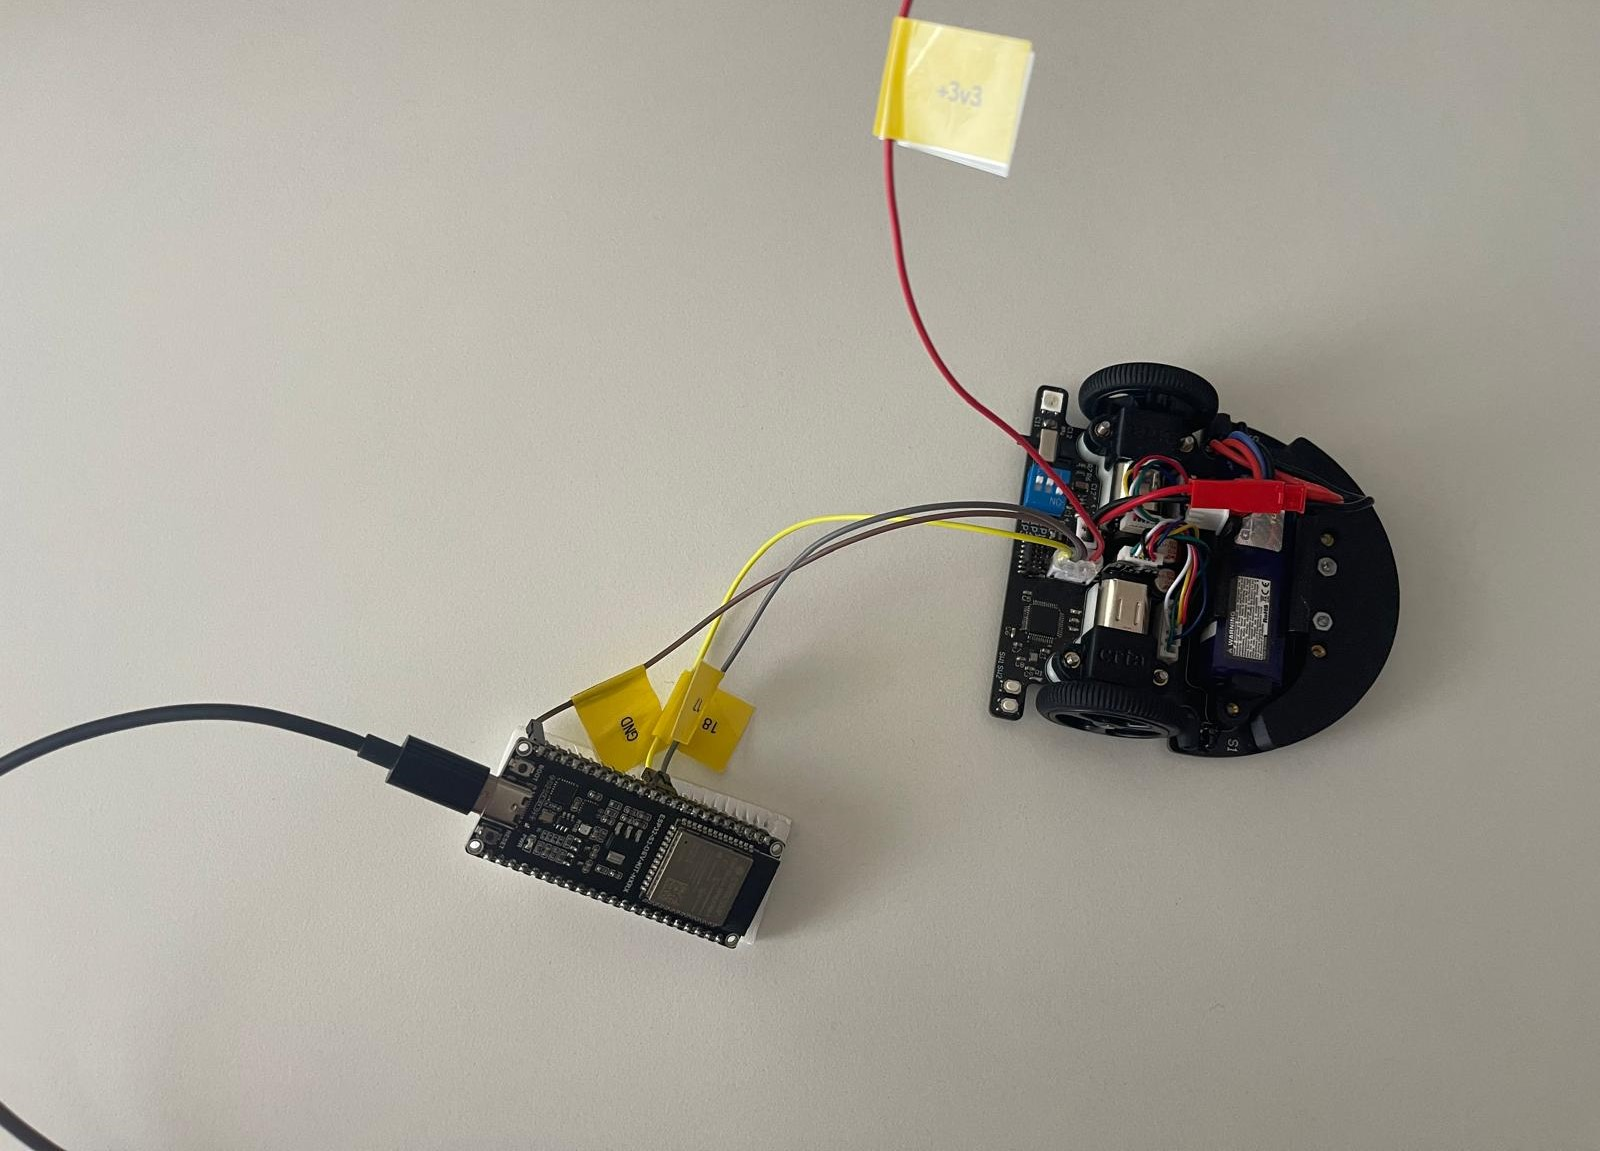
\includegraphics[width=0.75\textwidth]{slike/spoj.jpeg}
	\caption{Spoj ESP32 i robota preko UART-a (TX, RX, GND).}\label{fig:spoj}
\end{figure}

% -------------------------------------------------
\section*{5. Blok dijagram sustava}
% -------------------------------------------------

\begin{center}
	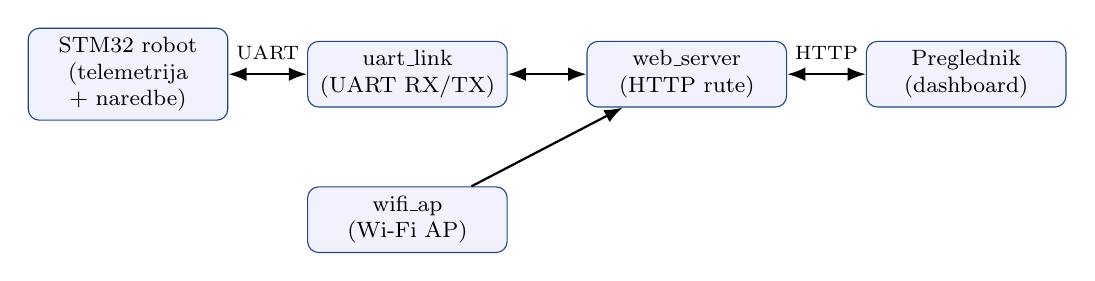
\begin{tikzpicture}[node distance=10mm and 10mm,
			block/.append style={text width=23mm,font=\footnotesize},
			lbl/.style={above,midway,font=\scriptsize,inner sep=5pt}]
		\node[block] (robot) {STM32 robot\\(telemetrija + naredbe)};
		\node[block,right=of robot] (uart) {uart\_link\\(UART RX/TX)};
		\node[block,right=of uart] (web) {web\_server\\(HTTP rute)};
		\node[block,below=of uart] (wifi) {wifi\_ap\\(Wi-Fi AP)};
		\node[block,right=of web] (browser) {Preglednik\\(dashboard)};

		\draw[line,Latex-Latex] (robot) -- node[lbl]{UART} (uart);
		\draw[line,Latex-Latex] (uart)  -- node[lbl]{} (web);
		\draw[line,Latex-Latex] (web)   -- node[lbl]{HTTP} (browser);
		\draw[line] (wifi) -- (web);
	\end{tikzpicture}
\end{center}

Blokovi:
\begin{itemize}
	\item \textbf{STM32 robot} -- šalje JSON telemetriju i izvršava primljene naredbe.
	\item \textbf{uart\_link} -- ESP-IDF komponenta; čita bajtove s UART-a, sastavlja linije i čuva zadnju primljenu liniju; šalje naredbe robotu.
	\item \textbf{wifi\_ap} -- podiže Wi-Fi pristupnu točku (SSID \texttt{Micromouse}, IP \texttt{192.168.4.1}).
	\item \textbf{web\_server} -- HTTP server koji poslužuje stranicu i posreduje telemetriju i naredbe.
	\item \textbf{Preglednik} -- prikazuje podatke i šalje naredbe; periodički dohvaća telemetriju.
\end{itemize}

% -------------------------------------------------
\section*{6. Programska struktura}
% -------------------------------------------------

Projekt je ESP-IDF aplikacija podijeljena na komponente. Svaka komponenta ima jednu odgovornost, što olakšava testiranje i izmjene neovisno o ostatku sustava.

\begin{table}[h!]
	\centering
	\begin{tabular}{@{}llp{8cm}@{}}
		\toprule
		\textbf{Cjelina} & \textbf{Datoteka}                                           & \textbf{Zadatak}                                                    \\
		\midrule
		Glavni program   & \texttt{main/main.c}                                        & inicijalizacija NVS-a i redom pokretanje AP-a, UART-a i web servera \\
		Wi-Fi AP         & \texttt{wifi\_ap.c/h}                                       & konfiguracija i pokretanje pristupne točke                          \\
		UART most        & \texttt{uart\_link.c/h}                                     & UART driver, RX task, slanje naredbi                                \\
		Web server       & \texttt{web\_server.c/h}                                    & HTTP server, ugrađene statičke datoteke, rute                       \\
		Frontend         & \texttt{index.html}, \texttt{script.js}, \texttt{style.css} & prikaz telemetrije i serijska konzola u pregledniku                 \\
		\bottomrule
	\end{tabular}
\end{table}

Statičke datoteke (\texttt{index.html}, \texttt{script.js}, \texttt{style.css}) ugrađene su u firmware preko \texttt{EMBED\_TXTFILES} u \texttt{CMakeLists.txt} web servera, pa nije potreban datotečni sustav na flashu.

% -------------------------------------------------
\section*{7. Flow dijagram}
% -------------------------------------------------

\begin{center}
	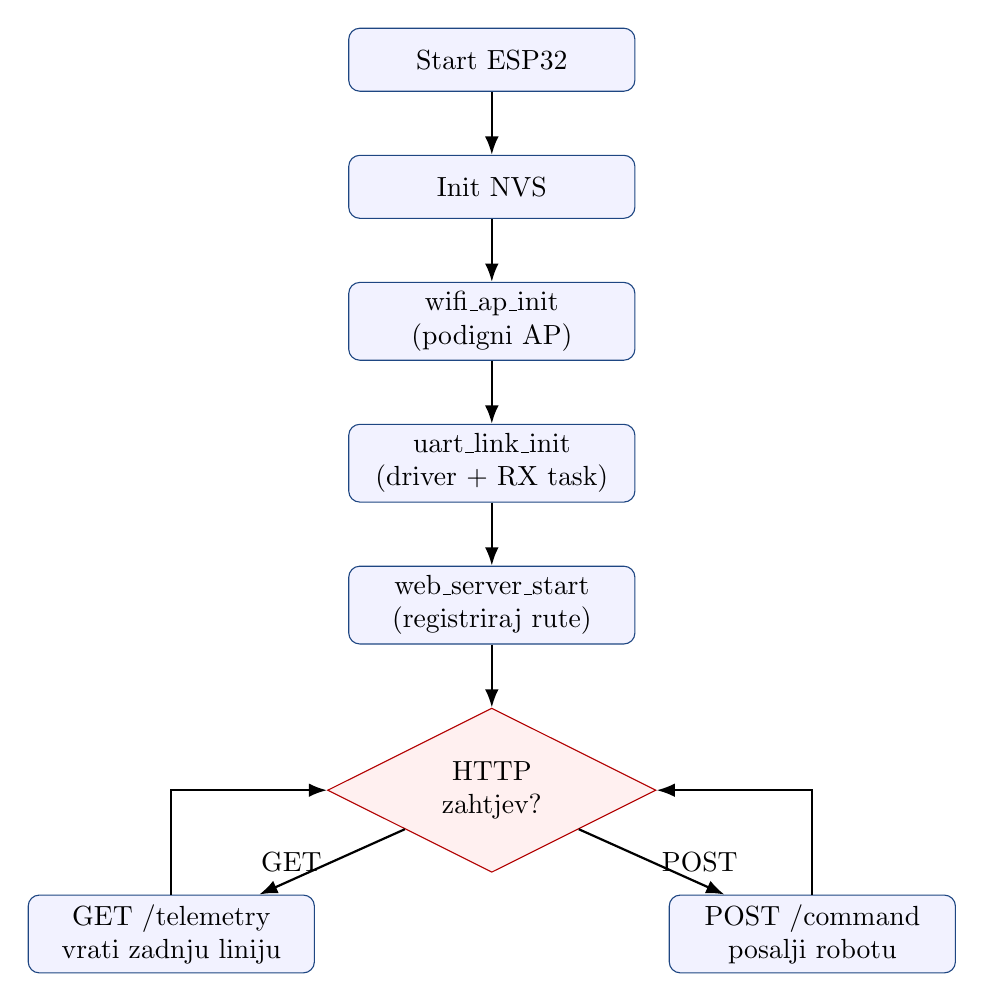
\begin{tikzpicture}[node distance=8mm]
		\node[block] (start) {Start ESP32};
		\node[block,below=of start] (nvs) {Init NVS};
		\node[block,below=of nvs] (ap) {wifi\_ap\_init\\(podigni AP)};
		\node[block,below=of ap] (uart) {uart\_link\_init\\(driver + RX task)};
		\node[block,below=of uart] (web) {web\_server\_start\\(registriraj rute)};
		\node[decision,below=of web] (event) {HTTP\\zahtjev?};
		\node[block,below left=8mm and 12mm of event] (telem) {GET /telemetry\\vrati zadnju liniju};
		\node[block,below right=8mm and 12mm of event] (cmd) {POST /command\\posalji robotu};

		\draw[line] (start) -- (nvs);
		\draw[line] (nvs) -- (ap);
		\draw[line] (ap) -- (uart);
		\draw[line] (uart) -- (web);
		\draw[line] (web) -- (event);
		\draw[line] (event) -- node[left]{GET} (telem);
		\draw[line] (event) -- node[right]{POST} (cmd);
		\draw[line] (telem) |- (event);
		\draw[line] (cmd) |- (event);
	\end{tikzpicture}
\end{center}

Najvažniji koraci:
\begin{itemize}
	\item NVS se inicijalizira jer ga Wi-Fi stog zahtijeva (kalibracije, MAC i sl.).
	\item RX task u pozadini neprestano čita UART i ažurira zadnju primljenu liniju.
	\item Web server je vođen zahtjevima: na \texttt{GET /telemetry} vraća zadnju liniju, na \texttt{POST /command} prosljeđuje naredbu robotu.
\end{itemize}

\pagebreak

% -------------------------------------------------
\section*{8. Pseudokod}
% -------------------------------------------------

\begin{lstlisting}[caption={Inicijalizacija (app\_main)}]
app_main:
    init NVS (erase + retry on error)
    wifi_ap_init()
    uart_link_init()
    web_server_start()
    log("Dashboard ready, http://192.168.4.1")
	\end{lstlisting}

\begin{lstlisting}[caption={RX task (sastavljanje linija s UART-a)}]
rx_task:
    loop forever:
        n = uart_read_bytes(chunk, timeout)
        for each byte c in chunk:
            if c is newline:
                if line not empty and line starts with '{':
                    commit_line(line)   # spremi pod mutexom
                reset line
            else if line not full:
                append c to line
            else:
                drop line (overflow)
	\end{lstlisting}

\begin{lstlisting}[caption={Preglednik (poll petlja)}]
every 50 ms:
    try:
        d = GET /telemetry           # JSON
        render(d)                    # popuni kartice
        status = "live"
    catch:
        status = "nema podataka"

on console Enter:
    cmd = input (lowercase, trimmed)
    if cmd == "clear": clear console
    else: POST /command  body=cmd
	\end{lstlisting}

% -------------------------------------------------
\section*{9. Web sučelje ili komunikacija}
% -------------------------------------------------

Korisnik se spoji na Wi-Fi mrežu \texttt{Micromouse} (lozinka \texttt{micromouse}, WPA2) i otvori \url{http://192.168.4.1}. Stranica je podijeljena na kartice (IR senzori, žiroskop, poza, odometrija, brzine, gibanje, tipke, DIP, Neopixel) i serijsku konzolu.

\textbf{HTTP rute (na ESP32):}

\begin{table}[h!]
	\centering
	\begin{tabular}{@{}lll@{}}
		\toprule
		\textbf{Ruta}       & \textbf{Metoda} & \textbf{Opis}                        \\
		\midrule
		\texttt{/}          & GET             & početna web stranica (HTML)          \\
		\texttt{/script.js} & GET             & klijentska logika                    \\
		\texttt{/style.css} & GET             & stilovi                              \\
		\texttt{/telemetry} & GET             & zadnja primljena telemetrija (JSON)  \\
		\texttt{/command}   & POST            & tijelo zahtjeva je naredba za robota \\
		\bottomrule
	\end{tabular}
\end{table}

\textbf{UART protokol.} Tekstualni je i jednostavan za debugiranje. Svaka poruka završava znakom za novi red. Telemetrija je jedna JSON linija; ESP prihvaća samo linije koje počinju znakom \texttt{\{} (osnovna validacija), a sve ostalo (debug ispisi robota) ignorira. Naredbe prema robotu su kratke tekstualne riječi.
\pagebreak

\textbf{Podržane naredbe:}
\begin{table}[h!]
	\centering
	\begin{tabular}{@{}ll@{}}
		\toprule
		\textbf{Naredba}     & \textbf{Učinak}                                            \\
		\midrule
		\texttt{reset\_odom} & resetira odometriju, enkodere i kut \texttt{yaw} na robotu \\
		\texttt{cycle\_led}  & uključuje/isključuje cikličko mijenjanje boje Neopixela    \\
		\texttt{clear}       & briše konzolu (obrađuje se samo u pregledniku)             \\
		\bottomrule
	\end{tabular}
\end{table}

\textbf{Primjer telemetrije (JSON odgovor na \texttt{/telemetry}):}

\begin{lstlisting}
{
  "ir": [120, 95, 30, 28, 88, 110],
  "gyro": { "Z": -1.25 },
  "Yaw": 12.430,
  "odom": { "Left": 1024, "Right": 1019 },
  "speed": { "Left": 3.14, "Right": 3.10 },
  "pose": { "X": 0.182, "Y": 0.004, "Theta": 0.217 },
  "v": 0.420, "w": 0.030,
  "btn": { "SW1": 0, "SW2": 1 },
  "dip": 5,
  "led": { "r": 0, "g": 100, "b": 0 }
}
	\end{lstlisting}

Polja: \texttt{ir} su 6 IR prijemnika (ADC očitanja),
\texttt{gyro.Z} kutna brzina po Z osi,
\texttt{Yaw} integrirani kut,
\texttt{odom} pozicija enkodera u tickovima,
\texttt{speed} brzine kotača,
\texttt{pose} poza robota,
\texttt{v}/\texttt{w} linearna i kutna brzina,
\texttt{btn} stanje tipki (1 = pritisnuto),
\texttt{dip} bitmaska 3 DIP prekidača,
\texttt{led} trenutna RGB boja Neopixela.
Polje \texttt{dip} se na klijentu rastavlja po bitovima (\texttt{dip >> i \& 1}).

% -------------------------------------------------
\section*{10. Testiranje}
% -------------------------------------------------

\begin{table}[h!]
	\centering
	\begin{tabular}{@{}p{5cm}p{5cm}p{3cm}@{}}
		\toprule
		\textbf{Test}                      & \textbf{Očekivani rezultat}                               & \textbf{Status} \\
		\midrule
		Pokretanje ESP32                   & U logu se vidi pokrenut AP i HTTP server                  & OK              \\
		Spoj na Wi-Fi i otvaranje stranice & Stranica se učita na \texttt{192.168.4.1}                 & OK              \\
		Prijem telemetrije                 & Kartice se ažuriraju, status pokazuje `live'              & OK              \\
		Odspajanje UART-a                  & Kartice prazne, status `nema podataka'                    & OK              \\
		Slanje \texttt{reset\_odom}        & Odometrija i \texttt{yaw} na robotu se postave na 0       & OK              \\
		Slanje \texttt{cycle\_led}         & Neopixel ledica na robotu se pali i ciklički mijenja boje & OK              \\
		Slanje \texttt{clear}              & Konzola u pregledniku se briše                            & OK              \\
		Neispravna linija na UART-u        & Linija bez \texttt{\{} se ignorira                        & OK              \\
		\bottomrule
	\end{tabular}
\end{table}

Dokazi rada prikazani su na slikama~\ref{fig:browser}--\ref{fig:serial}.

\begin{figure}[htbp]
	\centering
	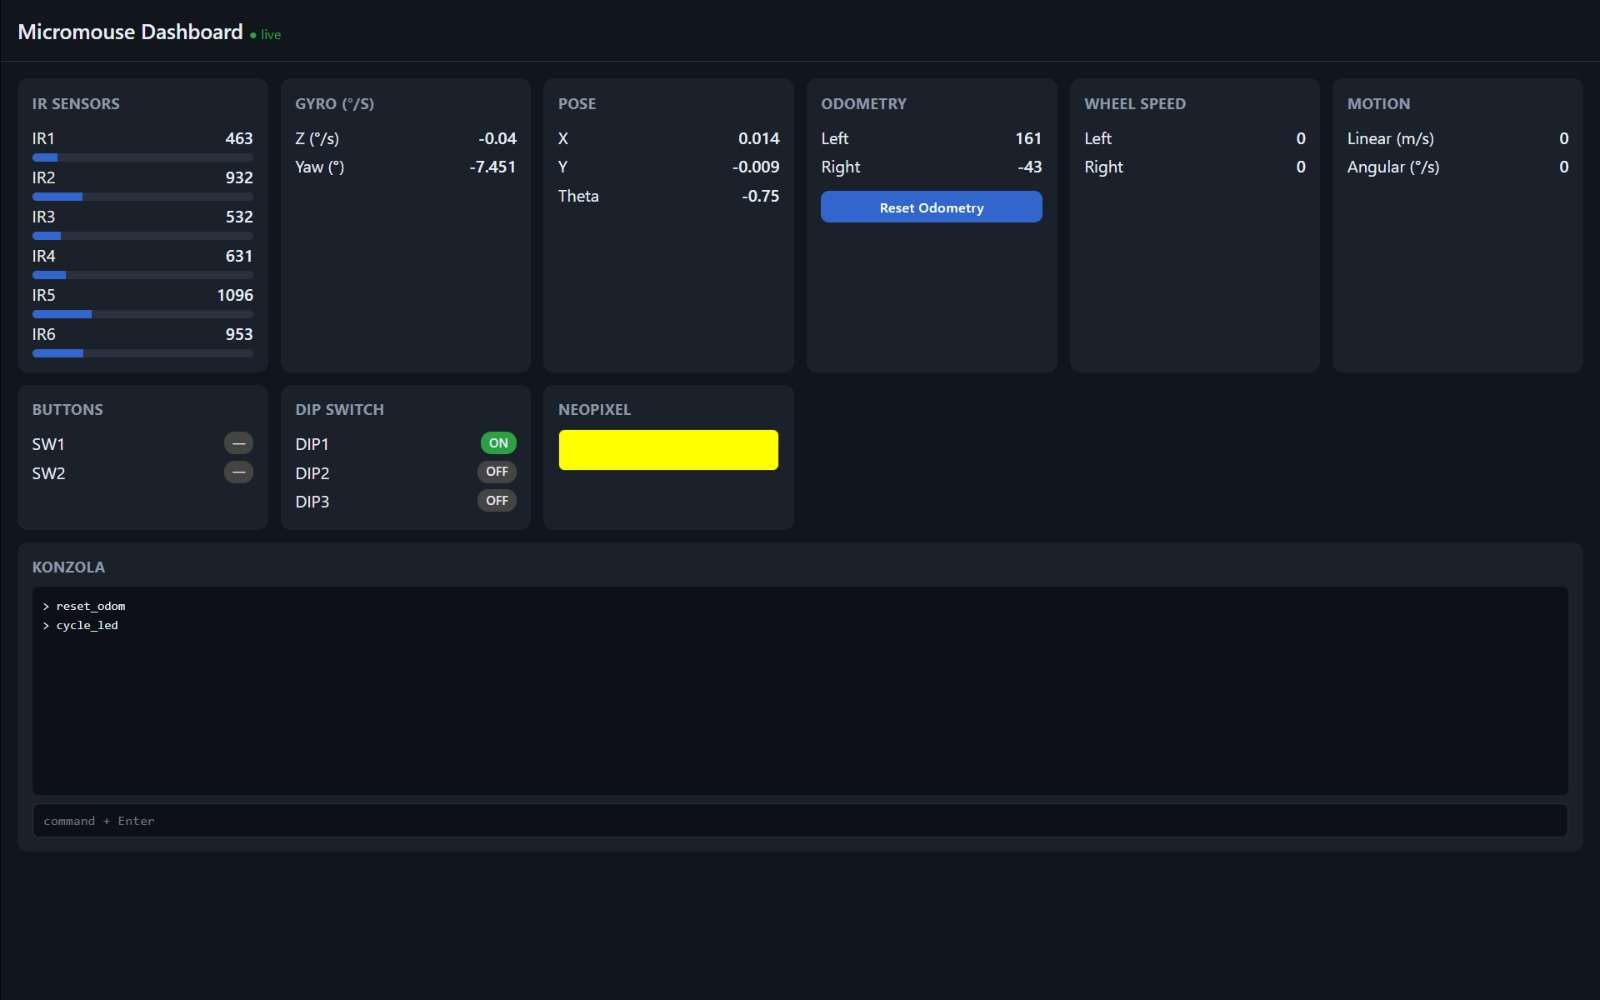
\includegraphics[width=0.75\textwidth]{slike/browser.jpeg}
	\caption{Web sučelje s aktivnom telemetrijom.}\label{fig:browser}
\end{figure}

\begin{figure}[htbp]
	\centering
	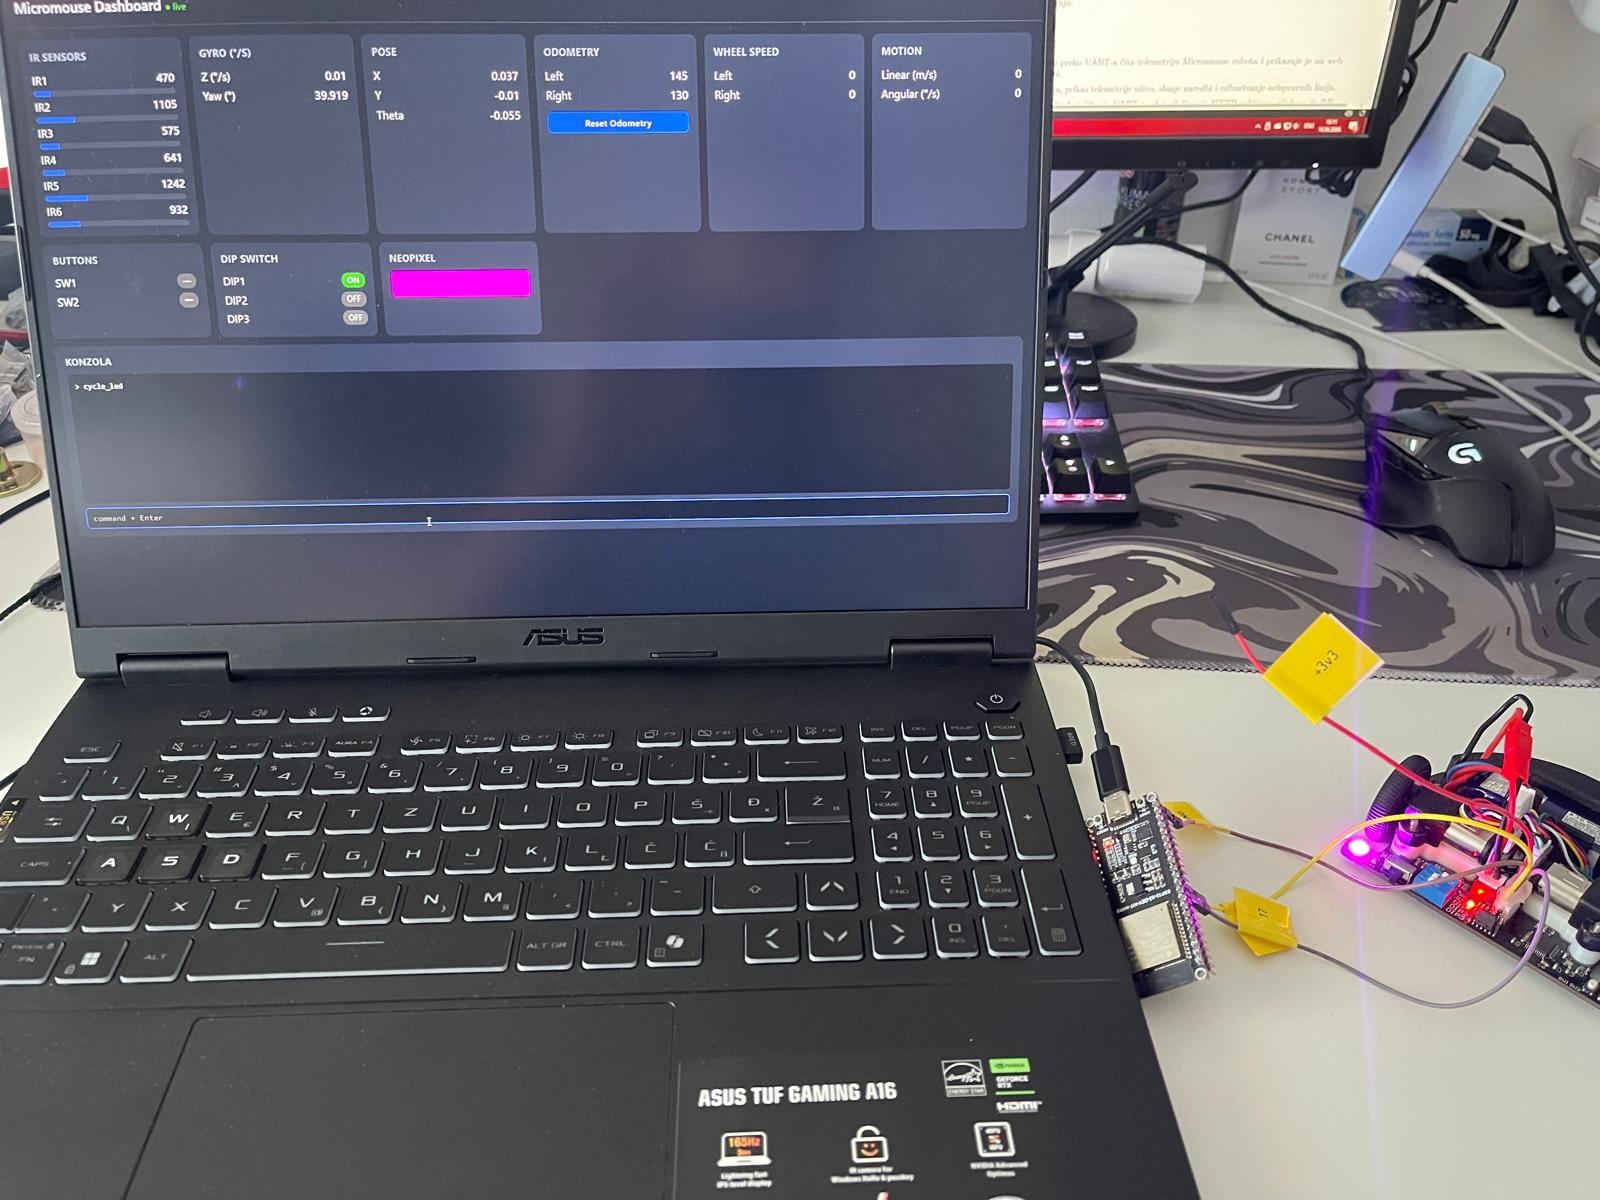
\includegraphics[width=0.6\textwidth]{slike/irl.jpeg}
	\caption{Laptop s pokrenutim dashboardom i robot pokraj njega.}\label{fig:irl}
\end{figure}

\begin{figure}[htbp]
	\centering
	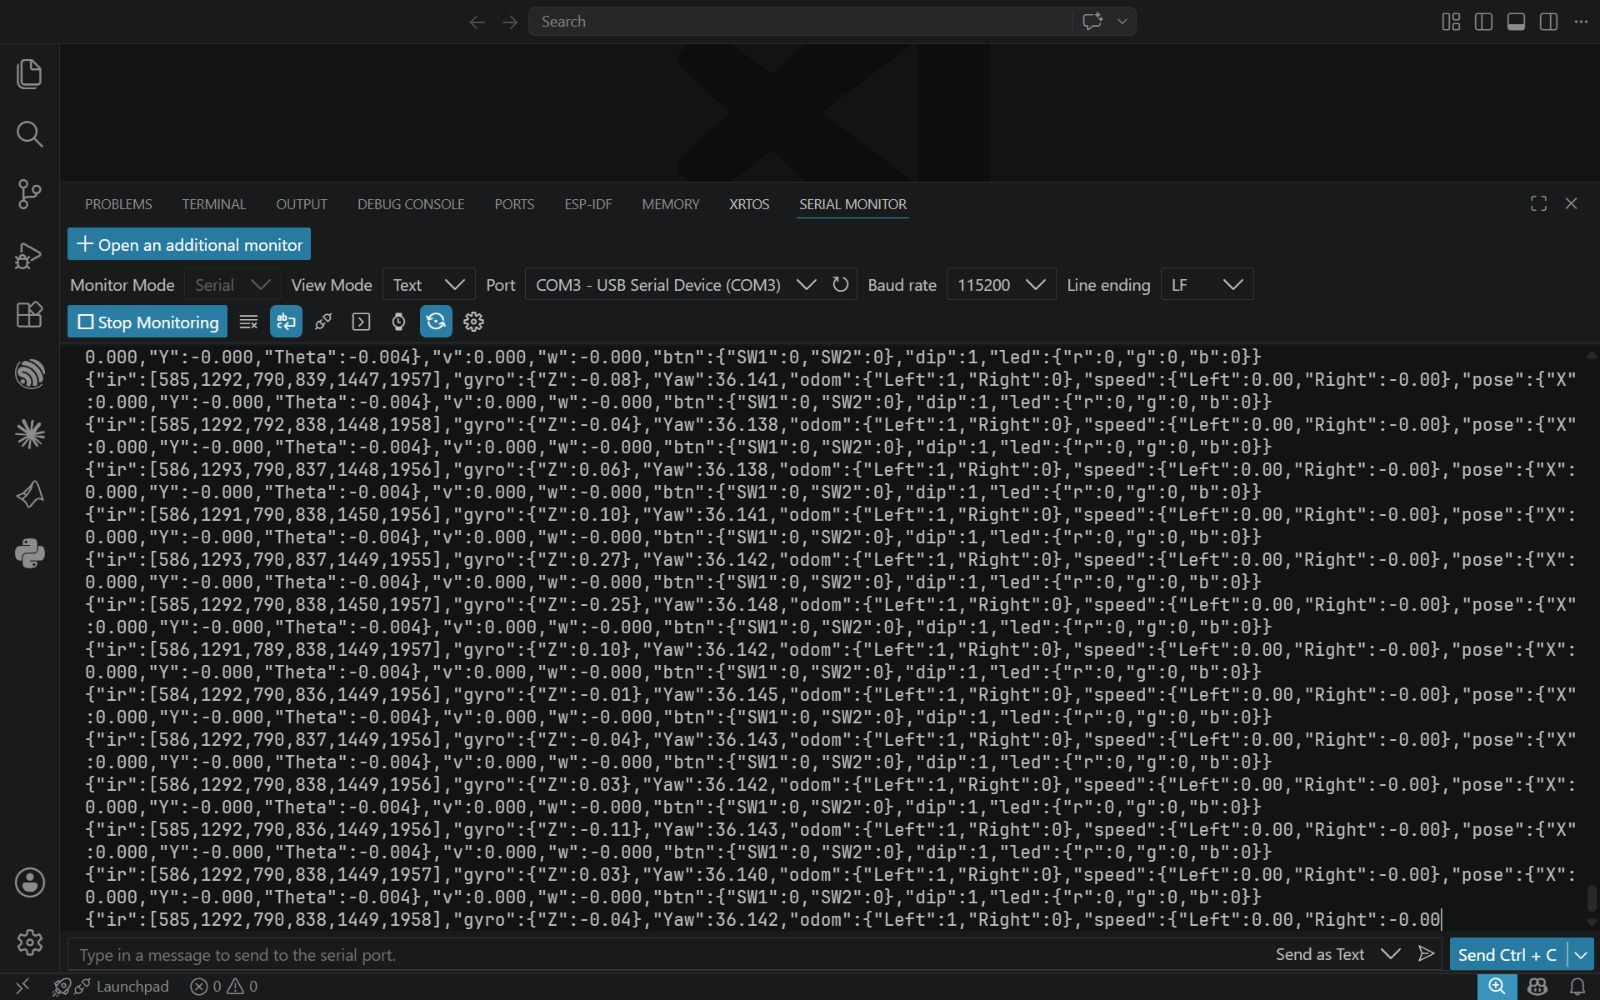
\includegraphics[width=0.6\textwidth]{slike/serial_monitor.jpeg}
	\caption{Ispis na serijski monitor.}\label{fig:serial}
\end{figure}

\pagebreak

% -------------------------------------------------
\section*{11. Zaključak}
% -------------------------------------------------

\begin{itemize}
	\item Napravljen je ESP32 dashboard koji preko UART-a čita telemetriju Micromouse robota i prikazuje je na web stranici, uz mogućnost slanja naredbi.
	\item Uspješno su testirani: podizanje AP-a, prikaz telemetrije uživo, slanje naredbi i odbacivanje neispravnih linija.
	\item Glavni izazov bio je odvajanje pozadinskog čitanja UART-a od posluživanja HTTP zahtjeva; riješeno je RX taskom i dijeljenjem zadnje linije pod mutexom.
	\item Moguća poboljšanja: detekcija gubitka veze po isteku vremena (npr. 5 s bez nove linije, a ne samo po HTTP grešci), pohrana postavki veze u NVS, te prelazak s pollinga na WebSocket radi manjeg opterećenja.
\end{itemize}

\end{document}
